% -*- coding: utf-8 -*-
% Paper Analysis Report — XeLaTeX Template
% Compile with: xelatex -interaction=nonstopmode <filename>.tex (run twice for TOC)
\documentclass[11pt, a4paper]{article}

% ============================================================
% Engine Detection & CJK Setup
% ============================================================
\usepackage{xeCJK}
\usepackage{fontspec}

% Chinese fonts
\setCJKmainfont[BoldFont={Noto Sans CJK SC Medium}]{Noto Serif CJK SC}
\setCJKsansfont{Noto Sans CJK SC}
\setCJKmonofont{Noto Sans Mono CJK SC}

% Latin fonts (referenced by filename for TeX tree discovery)
\setmainfont{texgyretermes}[
  Extension = .otf,
  UprightFont = *-regular,
  BoldFont = *-bold,
  ItalicFont = *-italic,
  BoldItalicFont = *-bolditalic
]
\setsansfont{texgyreheros}[
  Extension = .otf,
  UprightFont = *-regular,
  BoldFont = *-bold,
  ItalicFont = *-italic,
  BoldItalicFont = *-bolditalic
]
\setmonofont{texgyrecursor}[
  Extension = .otf,
  UprightFont = *-regular,
  BoldFont = *-bold,
  ItalicFont = *-italic,
  BoldItalicFont = *-bolditalic
]

% CJK spacing tuning
\xeCJKsetup{CJKmath=true, PlainEquation=true}

% ============================================================
% Page Layout
% ============================================================
\usepackage[
  a4paper,
  top=2.2cm, bottom=2.2cm,
  left=2.5cm, right=2.5cm,
  headheight=25pt
]{geometry}

\usepackage{setspace}
\setstretch{1.2}

% ============================================================
% Color Palette
% ============================================================
\usepackage[dvipsnames,svgnames,x11names]{xcolor}

\definecolor{PrimaryBlue}{HTML}{1A5276}
\definecolor{AccentTeal}{HTML}{148F77}
\definecolor{LightBg}{HTML}{F4F6F7}
\definecolor{DarkText}{HTML}{2C3E50}
\definecolor{SubtleGray}{HTML}{7F8C8D}
\definecolor{WarmOrange}{HTML}{E67E22}
\definecolor{CriticalRed}{HTML}{C0392B}
\definecolor{StrengthGreen}{HTML}{27AE60}
\definecolor{MathBlueBg}{HTML}{EBF5FB}
\definecolor{KeyBg}{HTML}{E8F8F5}

% ============================================================
% Section Styling
% ============================================================
\usepackage{titlesec}

\titleformat{\section}
  {\Large\bfseries\sffamily\color{PrimaryBlue}}
  {\thesection}{0.8em}{}
  [\vspace{-0.3ex}{\color{AccentTeal}\rule{\textwidth}{0.5pt}}]

\titleformat{\subsection}
  {\large\sffamily\color{PrimaryBlue!80!black}}
  {\thesubsection}{0.6em}{}

\titleformat{\subsubsection}
  {\normalsize\sffamily\color{PrimaryBlue!60!black}}
  {\thesubsubsection}{0.5em}{}

\titlespacing*{\section}{0pt}{2.5ex plus 1ex minus .2ex}{1.5ex plus .2ex}
\titlespacing*{\subsection}{0pt}{1.8ex plus 0.8ex minus .2ex}{0.8ex plus .2ex}
\titlespacing*{\subsubsection}{0pt}{1.2ex plus 0.5ex minus .1ex}{0.5ex plus .1ex}

% ============================================================
% Header & Footer
% ============================================================
\usepackage{fancyhdr}

\pagestyle{fancy}
\fancyhf{}
\fancyhead[L]{\small\sffamily\color{SubtleGray} \shorttitle}
\fancyhead[R]{}
\fancyfoot[C]{\small\sffamily\color{SubtleGray} --- \thepage{} ---}
\renewcommand{\headrulewidth}{0.4pt}
\renewcommand{\headrule}{\hbox to\headwidth{\color{AccentTeal!50}\leaders\hrule height \headrulewidth\hfill}}
\renewcommand{\footrulewidth}{0pt}

\fancypagestyle{plain}{
  \fancyhf{}
  \fancyfoot[C]{\small\sffamily\color{SubtleGray} --- \thepage{} ---}
  \renewcommand{\headrulewidth}{0pt}
}

% ============================================================
% Highlight Boxes (tcolorbox)
% ============================================================
\usepackage[most]{tcolorbox}

% Key insight / TL;DR box
\newtcolorbox{keyinsight}[1][核心要点]{
  enhanced,
  colback=KeyBg,
  colframe=AccentTeal,
  boxrule=0.6pt,
  left=10pt, right=10pt, top=8pt, bottom=8pt,
  arc=4pt,
  fonttitle=\bfseries\sffamily\small\color{AccentTeal},
  title={#1},
  shadow={1pt}{-1pt}{0pt}{AccentTeal!15},
  breakable
}

% Strength box
\newtcolorbox{strengthbox}[1][优势分析]{
  enhanced,
  colback=StrengthGreen!5,
  colframe=StrengthGreen!60!black,
  boxrule=0.4pt,
  left=8pt, right=8pt, top=6pt, bottom=6pt,
  arc=3pt,
  coltitle=white,
  fonttitle=\bfseries\sffamily\small,
  title={#1},
  breakable
}

% Weakness / critical box
\newtcolorbox{weaknessbox}[1][不足与局限]{
  enhanced,
  colback=CriticalRed!4,
  colframe=CriticalRed!50!black,
  boxrule=0.4pt,
  left=8pt, right=8pt, top=6pt, bottom=6pt,
  arc=3pt,
  coltitle=white,
  fonttitle=\bfseries\sffamily\small,
  title={#1},
  breakable
}

% Math / formula highlight box
\newtcolorbox{mathbox}[1][]{
  enhanced,
  colback=MathBlueBg,
  colframe=PrimaryBlue!40,
  boxrule=0.4pt,
  left=10pt, right=10pt, top=8pt, bottom=8pt,
  arc=3pt,
  breakable,
  title={#1},
  fonttitle=\bfseries\sffamily\small\color{PrimaryBlue}
}

% Info box (for metadata, reading suggestions, etc.)
\newtcolorbox{infobox}[1][]{
  enhanced,
  colback=LightBg,
  colframe=SubtleGray!60,
  boxrule=0.3pt,
  left=8pt, right=8pt, top=6pt, bottom=6pt,
  arc=3pt,
  breakable,
  title={#1},
  fonttitle=\bfseries\sffamily\small\color{DarkText}
}

% ============================================================
% Math, Algorithms, Tables
% ============================================================
\usepackage{amsmath, amssymb, amsthm}
\usepackage{algorithm}
\usepackage{algorithmic}
\usepackage{booktabs}
\usepackage{tabularx}
\usepackage{longtable}
\usepackage{multirow}
\usepackage{makecell}

% ============================================================
% Code Listings
% ============================================================
\usepackage{listings}
\lstset{
  basicstyle=\small\ttfamily\color{DarkText},
  backgroundcolor=\color{LightBg},
  frame=single,
  rulecolor=\color{SubtleGray!40},
  breaklines=true,
  numbers=left,
  numberstyle=\tiny\color{SubtleGray},
  keywordstyle=\color{PrimaryBlue}\bfseries,
  commentstyle=\color{StrengthGreen!70!black}\itshape,
  stringstyle=\color{WarmOrange},
  tabsize=4,
  xleftmargin=1em,
  framexleftmargin=0.5em
}

% ============================================================
% Hyperlinks & PDF Metadata
% ============================================================
\usepackage{hyperref}
\hypersetup{
  colorlinks=true,
  linkcolor=PrimaryBlue,
  citecolor=AccentTeal,
  urlcolor=AccentTeal!80!black,
  pdftitle={ARL-Tangram: Unleash the Resource Efficiency in Agentic Reinforcement Learning},
  pdfauthor={AI Research Analysis},
  bookmarksnumbered=true,
  bookmarksopen=true
}

% ============================================================
% Lists
% ============================================================
\usepackage{enumitem}
\setlist{nosep, leftmargin=1.5em}
\setlist[itemize,1]{label=\color{AccentTeal}\textbullet}
\setlist[itemize,2]{label=\color{PrimaryBlue!60}\textendash}

% ============================================================
% Graphics
% ============================================================
\usepackage{graphicx}
\usepackage{float}
\usepackage{subcaption}

% ============================================================
% Custom Commands
% ============================================================
\newcommand{\shorttitle}{}
\newcommand{\papertitle}[1]{%
  \renewcommand{\shorttitle}{#1}%
  \begin{center}
    \vspace*{0.3cm}
    {\small\sffamily\color{SubtleGray} 论文深度分析}\\[0.6em]
    {\LARGE\bfseries\sffamily\color{PrimaryBlue} #1}
  \end{center}
}
\newcommand{\paperauthors}[1]{%
  \begin{center}{\normalsize\color{DarkText} #1}\end{center}
}
\newcommand{\papervenue}[1]{%
  \begin{center}{\small\color{SubtleGray}\itshape #1}\end{center}
}
\newcommand{\paperdate}[1]{%
  \begin{center}{\small\color{SubtleGray} 分析日期：#1}\end{center}
}

\newcommand{\gmark}[1]{\textcolor{StrengthGreen!80!black}{\bfseries #1}}
\newcommand{\rmark}[1]{\textcolor{CriticalRed!80!black}{\bfseries #1}}
\newcommand{\omark}[1]{\textcolor{WarmOrange!80!black}{\bfseries #1}}

\newcommand{\ratingfull}{\textcolor{WarmOrange}{$\bigstar$}}
\newcommand{\ratinghalf}{\textcolor{WarmOrange!40}{$\bigstar$}}
\newcommand{\ratingempty}{\textcolor{SubtleGray!30}{$\bigstar$}}

% ============================================================
% Document Begin
% ============================================================
\begin{document}

\papertitle{ARL-Tangram: Unleash the Resource Efficiency\\in Agentic Reinforcement Learning}
\paperauthors{Bangjun Xiao, Yihao Zhao, Xiangwei Deng, Shihua Yu, Yuxing Xiang, Huaqiu Liu et al.\\
  School of Computer Science, Peking University \quad \& \quad LLM-Core Xiaomi}
\papervenue{arXiv:2603.13019v1 \quad | \quad 2026}
\paperdate{\today}

\vspace{0.8em}

\begin{keyinsight}[一句话总结]
ARL-Tangram 将智能体强化学习（Agentic Reinforcement Learning，ARL）中外部资源管理的粒度从轨迹级/任务级下沉至单次原子调用的 action 级，通过统一的资源建模、弹性调度算法与异构资源管理器，在真实 RL 训练任务上将平均 action 完成时间（Action Completion Time，ACT）提升最高~$4.3\times$，同时节省最多 71.2\% 的外部资源。
\end{keyinsight}

\vspace{0.5em}

{
  \hypersetup{linkcolor=DarkText}
  \tableofcontents
}

\newpage

% ============================================================
\section{论文元信息与分类}
% ============================================================

\begin{infobox}[论文信息]
\begin{tabular}{@{}p{2.8cm}p{10.5cm}@{}}
\textbf{标题} & ARL-Tangram: Unleash the Resource Efficiency in Agentic Reinforcement Learning \\[4pt]
\textbf{作者} & Bangjun Xiao$^{\dagger\ddagger}$, Yihao Zhao$^{\dagger\ddagger}$, Xiangwei Deng$^{\dagger\ddagger}$, Shihua Yu$^{\ddagger}$, Yuxing Xiang$^{\dagger\ddagger}$, Huaqiu Liu$^{\ddagger}$, Qiying Wang$^{\ddagger}$, Liang Zhao$^{\ddagger}$, Hailin Zhang$^{\ddagger}$, Xuanzhe Liu$^{\dagger}$, Xin Jin$^{\dagger}$, Fuli Luo$^{\ddagger}$ \\[4pt]
\textbf{机构} & $^\dagger$School of Computer Science, Peking University；$^\ddagger$LLM-Core Xiaomi \\[4pt]
\textbf{发表/预印} & arXiv:2603.13019v1，2026年3月13日 \\[4pt]
\textbf{论文类型} & 系统设计与实现 \\[4pt]
\textbf{核心领域} & Systems, Distributed Computing, Reinforcement Learning \\
\end{tabular}
\end{infobox}

\vspace{0.8em}

\textbf{一句话定位}：本文针对云端智能体 RL 训练中外部资源严重过度供给（over-provisioning）的痛点，提出了 action 级别的统一外部资源调度系统 ARL-Tangram，并将其部署于小米 MiMo 系列模型的训练流程中。

% ============================================================
\section{核心摘要与定性评估}
% ============================================================

\begin{keyinsight}[TL;DR]
与传统 RL 不同，智能体 RL 需要大量位于主训练集群之外的外部资源（CPU、GPU、API quota），而现有框架的静态 over-provisioning 导致这些资源严重浪费。ARL-Tangram 将管理粒度细化到单次原子调用（action），通过弹性调度最大化资源利用率，在真实生产任务上显著降低 ACT 并节省资源成本。
\end{keyinsight}

\begin{figure}[htbp]
\centering
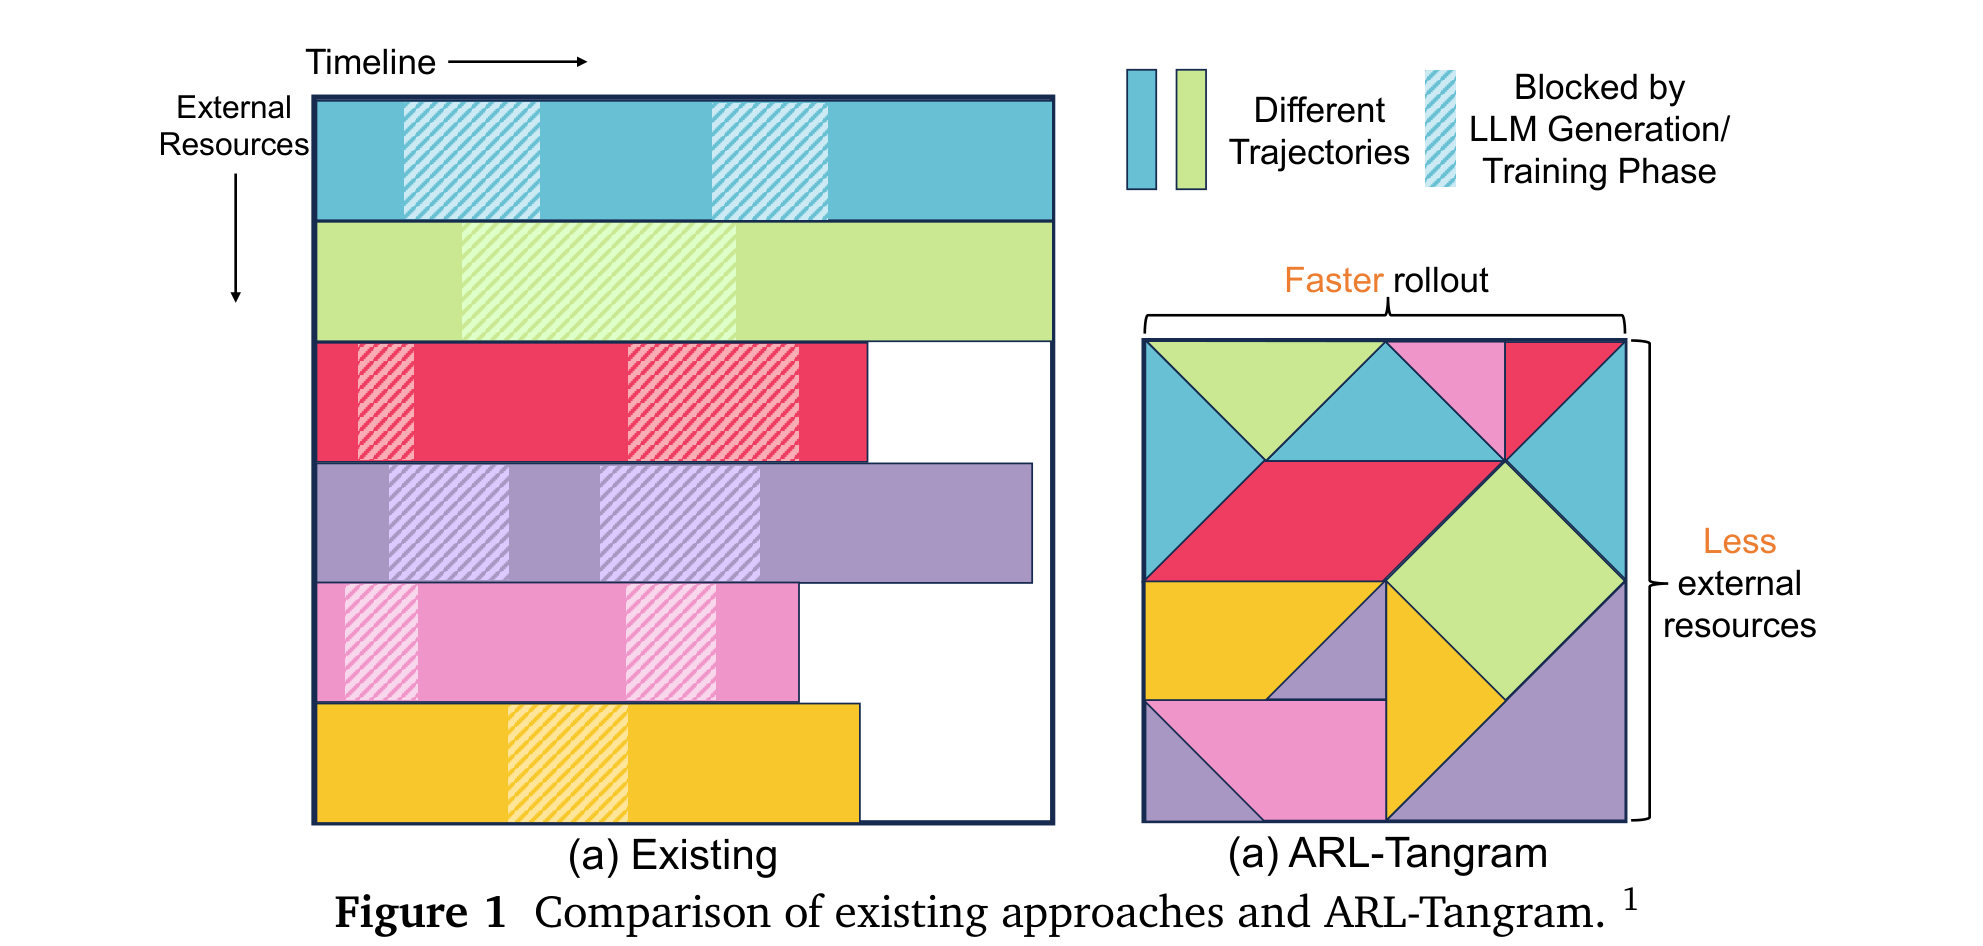
\includegraphics[width=0.92\textwidth]{figures/fig1.png}
\caption{现有方法与 ARL-Tangram 的资源管理策略对比。现有框架静态预分配外部资源（离线优化阶段），导致 RL 生成训练阶段资源大量空置；ARL-Tangram 通过 action 级动态调度实现跨轨迹、跨任务的弹性共享。}
\label{fig:comparison}
\end{figure}

\subsection{技术摘要}

智能体 RL（Agentic Reinforcement Learning，ARL）的 rollout 阶段需要反复调用位于主 GPU 训练集群之外的异构外部资源——AI coding 任务需要 CPU 集群执行代码、DeepSearch 需要消耗 API quota，而奖励计算往往依赖独立部署的 GPU reward model。然而现有 RL 框架对外部资源的管理停留在轨迹（trajectory）级或任务（task）级的静态预分配，导致两个层次的过度供给：（1）轨迹级——环境仅在 47\% 的轨迹生命周期内被使用，而 CPU 资源在整个 rollout 期间始终被占用；（2）任务级——不同 RL 任务各自独占外部服务，而这些服务在训练阶段（LLM 训练时）完全空闲，调用次数的波动高达三个数量级。

ARL-Tangram 提出 action 级调度（action-level scheduling），将外部资源从长生命周期的环境/服务中 breakdown（释放后复用），并通过资源池化（pool）在不同轨迹和任务间弹性共享。系统核心包括：（1）统一的向量化资源代价建模，支持多维资源约束与弹性度建模；（2）基于贪心淘汰的弹性调度算法，以最小化全局 ACT 为目标；（3）针对 CPU 和 GPU 的异构资源管理器，分别引入 allocate-on-execution（AOE）和 evict-on-execution（EOE）机制。在真实 agentic RL 任务上，ARL-Tangram 将平均 ACT 提升最高~$4.3\times$，RL 训练 step 时长缩短最高~$1.5\times$，外部资源节省最高 71.2\%，并已在小米 MiMo 系列模型训练中投入生产。

\begin{keyinsight}[贡献完整性核查]
原文 abstract 列举的四项核心贡献均在摘要中得到覆盖：（1）over-provisioning 问题分析与分类；（2）action 级调度框架 ARL-Tangram；（3）统一 action formulation 与弹性调度算法；（4）真实任务评估结果。同时，系统部署于 MiMo 系列模型这一工业落地贡献亦有记录。
\end{keyinsight}

\subsection{定性评估矩阵}

\begin{table}[htbp]
\centering
\caption{定性评估}
\label{tab:qualeval}
\begin{tabular}{llp{0.52\textwidth}}
\toprule
\textbf{评估维度} & \textbf{评级} & \textbf{说明} \\
\midrule
新颖性 & 中等创新 & action 级调度思想在云计算中并非首创，但将其系统性地应用于 agentic RL 的外部资源管理是新颖的，Breakdown \& Pool 的组合机制具有实用价值 \\
技术严谨性 & 高 & 算法部分有明确的数学形式化，AOE/EOE 机制有深入的系统设计；实验使用真实生产 workload \\
实验充分性 & 充分 & 覆盖三种 workload、多种 batch size、scalability 和消融实验；缺乏统计显著性报告 \\
可复现性 & 中 & 系统设计细节描述充分，但代码未开源；testbed 为私有生产集群，无法直接复现 \\
写作质量 & 良好 & 结构清晰，问题动机充分，图表设计直观 \\
\bottomrule
\end{tabular}
\end{table}

\subsection{与原文摘要的对比}

原文摘要的数据引用精确，未发现明显夸大。以下几点值得注意：

\begin{itemize}
  \item 「平均 ACT 提升最高~$4.3\times$」来自 AI Coding workload 的 total 外部调用时间（环境交互~$9.0\times$ + 奖励计算~$2.8\times$ 的综合效果），在 MOPD workload 上改善幅度更小，摘要未加说明。
  \item 「step duration 缩短~$1.5\times$」仅对 AI Coding 和 DeepSearch 成立；MOPD 的 step duration 改善相对较小（受 long-tail trajectory 主导）。
  \item 「节省 71.2\% 外部资源」来自 GPU 资源的特定场景（10 个 reward service 仅需 29\% GPU），是特定实验配置下的最优结果。
\end{itemize}

% ============================================================
\section{创新贡献与研究定位}
% ============================================================

\begin{keyinsight}[TL;DR]
ARL-Tangram 的核心创新在于将云计算资源调度的细粒度思想与 agentic RL 的异构外部资源需求系统性地结合，通过基础设施层面的 Breakdown \& Pool 机制和针对 CPU/GPU 异构拓扑的专用管理器，填补了现有 RL 框架在外部资源管理上的空白。
\end{keyinsight}

\subsection{技术贡献清单}

\begin{enumerate}
  \item \textbf{[算法] 弹性 action 级调度算法}：提出以最小化 ACT 为目标的贪心淘汰（greedy eviction）调度算法，融合 FCFS 执行顺序策略与向量化资源弹性建模，支持异构资源约束下的并发 action 弹性资源分配。算法复杂度~$O(kn^2m^2)$，适配高并发短时延场景。

  \item \textbf{[基础设施] ARL-Tangram 统一资源管理系统}：设计并实现了独立于 RL 框架、外部资源类型、调用类型的通用 action 级资源管理平台，包含统一 action formulation 模块、弹性调度器和标准化异构资源接口，已在小米生产集群中部署支持 MiMo 系列模型训练。

  \item \textbf{[工程] CPU Manager via AOE（Allocate-on-Execution）}：利用 Docker 的 cgroup 接口在每次 action 执行前动态更新容器的 cpulimit 和 cpuset，实现 CPU 资源在 action 粒度的 breakdown 与弹性 DoP 支持，同时保留容器内存以维持长生命周期环境状态。CPU 分配策略优先在同一 NUMA 节点内选核以降低跨核通信开销。

  \item \textbf{[工程] GPU Manager via EOE（Evict-on-Execution）}：针对 GPU reward service 的高初始化开销（kernel 编译、通信组建立、模型参数加载），设计 CPU 内存备份 + LRU 淘汰的 GPU 显存管理机制，结合多级 chunk 结构（大小为~$\{1, 2, 4, 8\}$，满足~$2^a$ 对齐约束）减少 GPU 内存碎片，支持 multi-service 弹性 DoP 共享同一 GPU 集群。

  \item \textbf{[工程] 拓扑无关的 DPArrange 动态规划算法}：为弹性调度器提供最优离散资源分配的底层 DP 求解器，通过 DP Operator 接口屏蔽不同资源拓扑（CPU 线性拓扑、GPU chunk 拓扑）的差异，实现调度算法的拓扑透明性。
\end{enumerate}

\subsection{研究脉络定位}

ARL-Tangram 所处的研究交叉点涵盖三个方向：

\paragraph{RL 框架优化}
OpenRLHF（Hu et al., 2024）和 verl（Sheng et al., 2025）分别探索了 disaggregated 和 colocated 的 RL 框架架构，后续工作在 fusion、pipelining、streaming 和异步执行等方向持续优化。这些框架均聚焦于主 GPU 训练集群的效率，对外部资源的管理或忽略、或沿用静态 over-provisioning 策略。

\paragraph{智能体资源管理}
Mars（Zhu et al., 2026）首次将 reward 计算抽象为独立服务，利用 request-in, batch-out 特性放松延迟约束。MegaFlow（Zhang et al., 2026）、SkyRL-Agent（Cao et al., 2025）和 ROCK（Wang et al., 2025a）将 cloud computing 技术引入 agent 服务管理，但均未提供统一的 action 级弹性调度框架。

\paragraph{云计算资源自动伸缩}
传统 LLM serving 中的 autoscaling 工作（Xiang et al., 2025；Zhang et al., 2025）针对 inference workload 的 SLO 进行优化。ARL-Tangram 将弹性分配引入 RL rollout 的 action 粒度，与以上工作在目标函数和场景上均有本质差异。

\textbf{填补的研究空白}：现有工作要么优化 RL 框架本身、要么针对单类外部资源，没有提供跨异构资源类型、支持多维弹性约束、面向 agentic RL 全流程的统一外部资源调度方案。

\subsection{与最近似工作的深度对比}

\begin{table}[htbp]
\centering
\caption{ARL-Tangram 与近似工作的技术对比}
\label{tab:comparison}
\begin{tabular}{p{2.8cm}p{3.2cm}p{3.2cm}p{3.2cm}}
\toprule
\textbf{维度} & \textbf{ARL-Tangram} & \textbf{Mars (Zhu et al., 2026)} & \textbf{ServerlessLLM (Fu et al., 2024)} \\
\midrule
管理对象 & 全类型外部资源（CPU、GPU、API quota） & 仅 reward 计算服务 & LLM inference 服务 \\
调度粒度 & Action 级（单次原子调用） & Batch 级 & Request 级 \\
弹性机制 & 向量化多维资源弹性 DoP & 历史 based scaling + timeout & 模型-as-a-Service 多模型复用 \\
GPU 管理 & EOE + LRU + chunk 结构 & 未详述 & Serverless 冷启动优化 \\
CPU 管理 & AOE + Docker cgroup + NUMA aware & 不涉及 & 不涉及 \\
RL 集成 & 与 RL 框架解耦，独立系统 & 与 RL 框架耦合 & 面向通用 LLM serving \\
生产部署 & 已部署（MiMo 系列训练） & 原文未提及 & USENIX OSDI 2024 论文工作 \\
\bottomrule
\end{tabular}
\end{table}

% ============================================================
\section{研究背景与问题形式化}
% ============================================================

\begin{keyinsight}[TL;DR]
Agentic RL 将 LLM 与真实世界工具调用结合，使得 RL 训练对外部资源的依赖远超传统 RL，而云端资源管理领域成熟的弹性调度机制尚未被引入这一场景。
\end{keyinsight}

\subsection{技术背景与现状}

\paragraph{Agentic RL 的资源需求特征}
与传统 LLM RL（仅消耗 GPU）不同，agentic LLM 通过 shell command、API 调用或设备操作与外部环境交互。在 rollout 阶段，LLM 遵循 ReAct 模式（Yao et al., 2022）反复交替生成（GPU）和工具调用（外部资源），形成 multi-turn 轨迹。这意味着外部资源调用（tool invocation 和 reward 计算）均处于每个样本的关键路径上，其延迟直接影响整体 rollout 吞吐。

\paragraph{外部资源的多样性}
\begin{itemize}
  \item \textbf{CPU 集群}：AI coding 任务需要隔离的执行环境（Docker 容器）来运行代码并评估测试用例；
  \item \textbf{GPU 集群}：reward model 推理（如 LLM-as-a-judge、MOPD 中的教师模型）需要独立的 GPU 服务；
  \item \textbf{外部 API}：DeepSearch 需要消耗 Google Search 等 web 搜索 API quota。
\end{itemize}

\paragraph{现有 RL 框架的局限}
以 VeRL（Sheng et al., 2025）为代表的现有 RL 框架将外部资源管理默认为静态 over-provisioning：每条轨迹独占一个 pod（k8s 分配），整个 rollout 生命周期内保持预留；不同 RL task 各自独立部署外部服务实例，不跨任务共享。

\subsection{核心技术挑战}

\paragraph{挑战一：轨迹级 over-provisioning}
AI coding 任务中，每条轨迹平均仅 47\% 的生命周期内实际访问外部资源，其余时间（LLM 生成和训练阶段）CPU 资源被空置浪费（浪费比例约 53\%）。在 finite resources 约束下，这严重限制了系统并发度，增加 tool invocation 的排队延迟。

\paragraph{挑战二：任务级 over-provisioning}
MOPD workload 使用 12 个教师模型 reward service，GPU SM activity 平均不足 3\%，振荡剧烈（Figure 3(b)）。外部调用次数在整个训练过程中波动高达三个数量级（Figure 3(d)），导致服务在大部分时间严重欠载。

\begin{figure}[htbp]
\centering
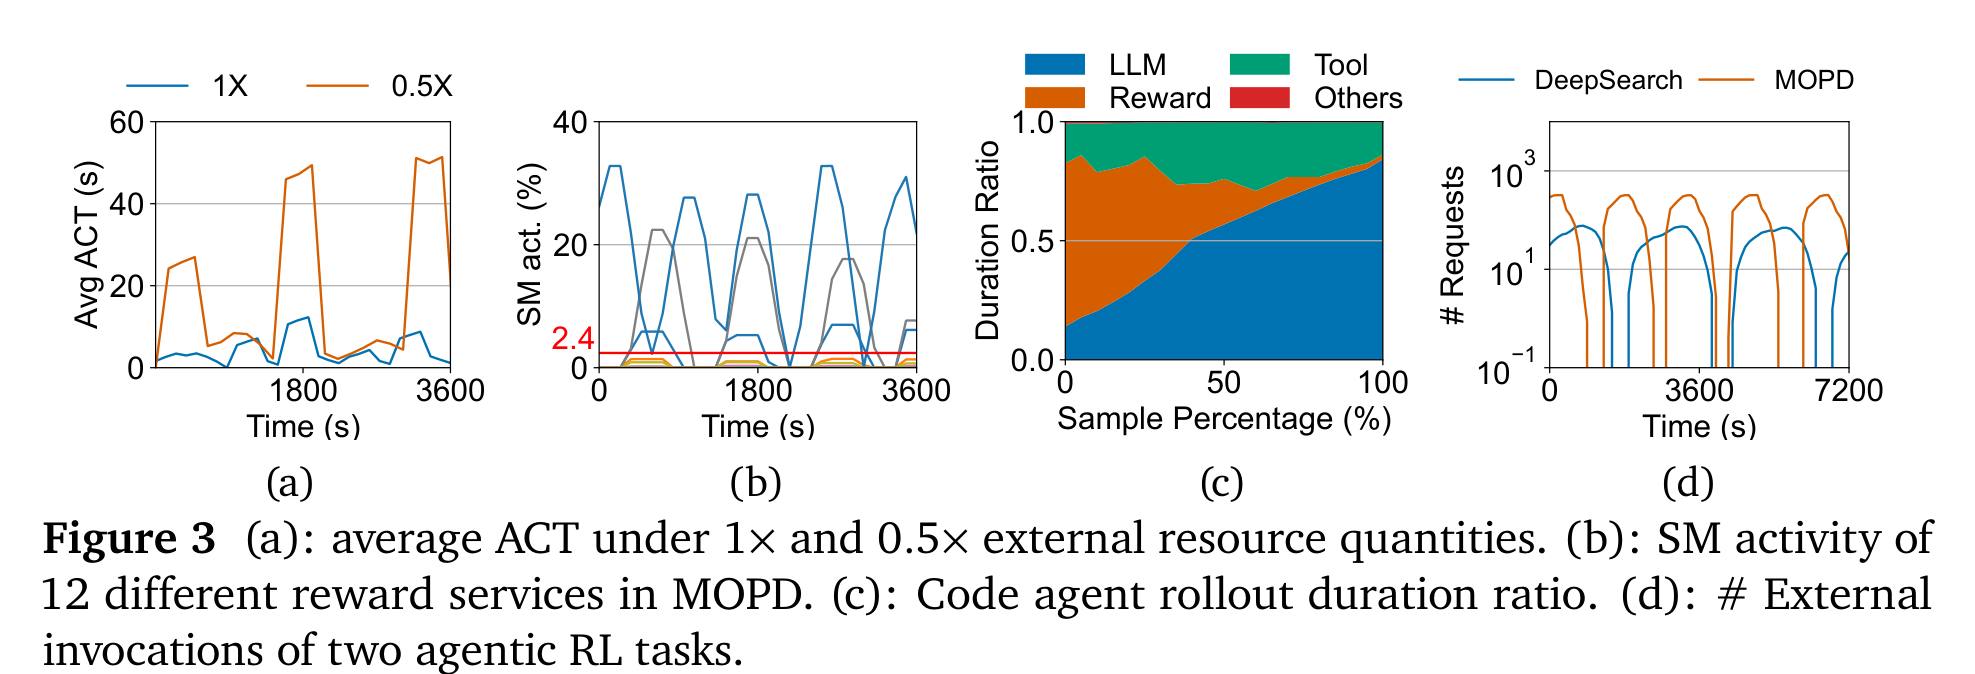
\includegraphics[width=\textwidth]{figures/fig3.png}
\caption{过度供给问题的量化分析（AI coding 和 MOPD workload）。(a) 外部资源数量与 ACT 的关系；(b) GPU SM 活跃度（MOPD reward service 平均不足 3\%）；(c) 各阶段耗时比例（LLM 生成与训练期间外部资源空置率达 53\%）；(d) 单 step 内外部调用次数（波动高达三个数量级）。}
\label{fig:motivation}
\end{figure}

\paragraph{挑战三：action 级调度的实现复杂性}
（1）不同 action 的资源需求类型各异，部分 action 需要同时消耗多种资源；（2）调度窗口极短（AI coding 中 action 执行时间可短至 1ms），无法使用重量级优化算法；（3）需要在不中断长生命周期状态（环境文件系统、模型参数）的前提下实现资源的按需分配。

\subsection{问题形式化}

\begin{mathbox}[ACT 最小化目标函数]
令~$N$ 为等待队列中的 action 数量，$T_i^q$ 为第~$i$ 个 action 的排队时延，$T_i$ 为其实际执行时延，则 elastic resource scheduling 的优化目标为：
\begin{equation}
  \text{minimize} \quad \mathit{ACT}_s = \sum_{0 \leq i < N} \left( T_i^q + T_i \right)
  \label{eq:act}
\end{equation}
subject to：$\forall j \in \{0, \ldots, k-1\}$，资源类型~$j$ 的分配满足向量化约束~$R_j \geq \{c^{\min}_{0,j}, \ldots, c^{\min}_{n-1,j}\}$（其中~$\geq$ 不仅要求总量满足，还要求实际拓扑能够容纳所有 candidate）。
\end{mathbox}

对于弹性 action，执行时延与分配资源量的关系由弹性函数给出：
\begin{equation}
  a.\mathit{getDur}(m) = \frac{T_{\mathit{ori}}}{E(m) \cdot m}, \quad 0 < E(m) \leq 1
  \label{eq:elasticity}
\end{equation}
其中~$T_{\mathit{ori}}$ 为分配单个 unit 时的基准执行时长，$E(m)$ 为弹性比（efficiency ratio），描述分配~$m$ 个 unit 时的并行效率。$E(m) = 1$ 代表线性加速，$E(m) < 1$ 表示存在并行开销。

\subsection{研究空白分析}

现有工作的核心空白在于：没有任何系统将 agentic RL 的外部资源管理统一到 action 粒度，并同时支持 CPU 和 GPU 两类异构外部资源的弹性共享。Mars 仅处理 reward service，ServerlessLLM 针对通用 LLM serving 而非 RL rollout 的 bursty 特征，Kubernetes 的 pod 级管理粒度与 action 级需求之间存在根本的粒度错配。

% ============================================================
\section{技术方法与系统架构}
% ============================================================

\begin{keyinsight}[TL;DR]
ARL-Tangram 是一个三层架构系统：统一 action formulation 层负责异构资源建模，弹性调度层基于贪心淘汰算法最小化 ACT，异构资源管理层通过 AOE（CPU）和 EOE（GPU）实现 action 粒度的资源 breakdown 与 pool。
\end{keyinsight}

\subsection{整体架构}

如图~\ref{fig:overview} 所示，ARL-Tangram 作为集中式中间层，解耦了 RL tasks 与异构外部资源之间的直接依赖。系统的标准执行循环包含五个阶段：

\begin{enumerate}
  \item \textbf{Action Submission}：rollout 期间，agentic LLM 每次发起工具调用或 reward 请求时，提交至 ARL-Tangram；
  \item \textbf{Unified Formulation \& Queuing}：formulation 模块将各类外部资源调用转换为统一的 action 表示，提交至统一的 Action Waiting Queue；
  \item \textbf{Elastic Scheduling}：调度器在外部资源约束下调度等待队列中的 action，与各 Resource Manager 协作弹性分配资源；
  \item \textbf{Action Execution}：各 action 在相应 Resource Manager 分配的资源上独立执行；
  \item \textbf{Transmit \& Observation}：执行完成后，结果返回 RL 框架，LLM 继续下一轮生成。
\end{enumerate}

\begin{figure}[htbp]
\centering
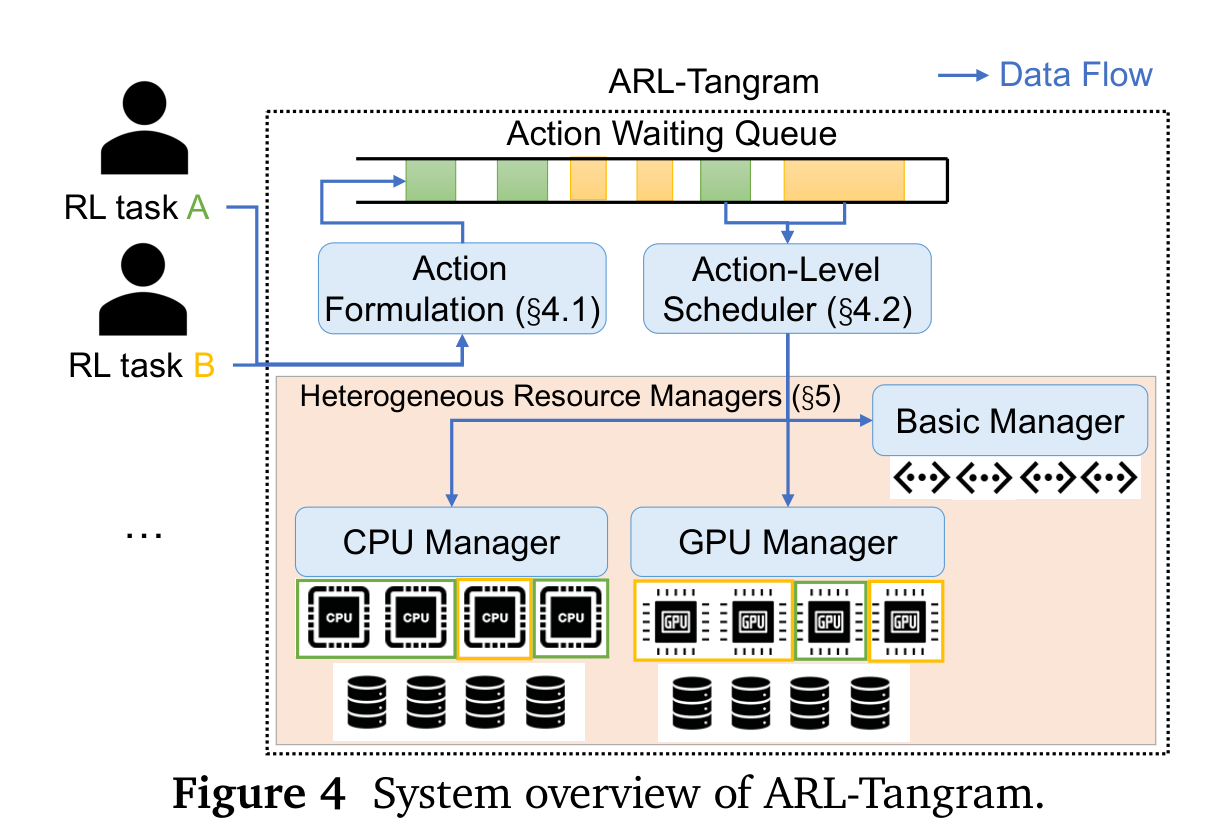
\includegraphics[width=0.85\textwidth]{figures/fig4.png}
\caption{ARL-Tangram 系统整体架构。系统作为中间层解耦 RL tasks 与异构外部资源，核心组件为 Action Formulation 模块、弹性调度器和三类 Resource Manager（CPU Manager、GPU Manager、Basic Manager）。}
\label{fig:overview}
\end{figure}

\begin{figure}[htbp]
\centering
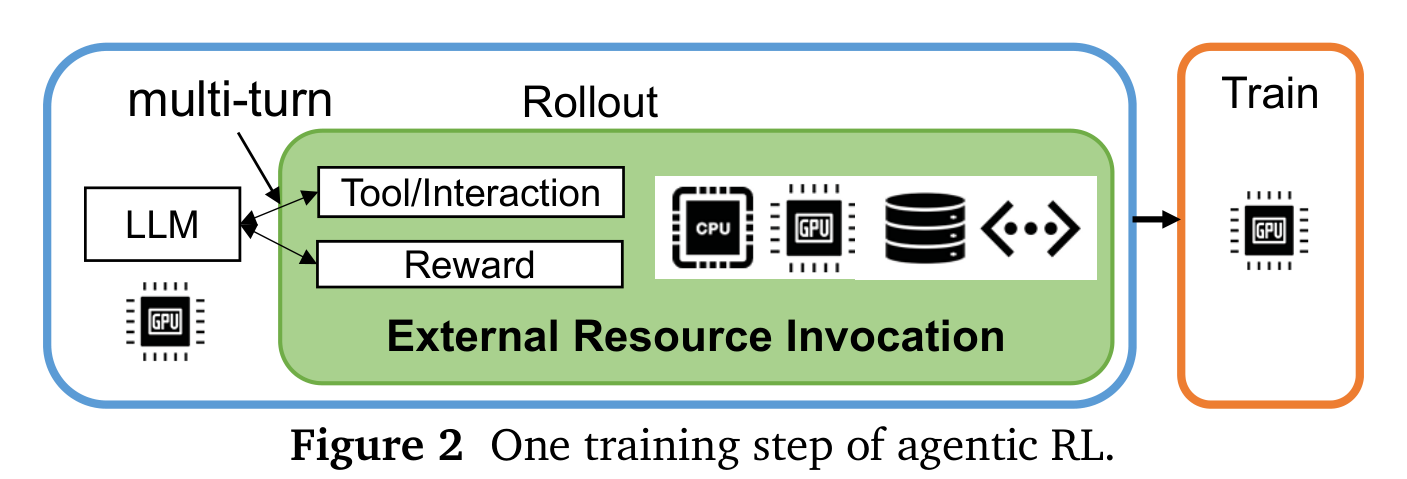
\includegraphics[width=0.85\textwidth]{figures/fig2.png}
\caption{单步 agentic RL 训练流程。Rollout 阶段中，LLM 生成（GPU）与外部资源调用（Tool/Reward，占用外部 CPU 或 GPU）交替进行，外部调用均处于每个 sample 的关键路径上。}
\label{fig:training-step}
\end{figure}

\subsection{关键组件深入分析}

\subsubsection{Action Formulation：统一的异构资源建模}

\paragraph{向量化资源代价建模}
给定 action~$a_i$，其资源代价表示为~$k$ 维向量：
\[
  C_i = (c_{i,0},\, c_{i,1},\, \ldots,\, c_{i,k-1})
\]
其中~$k$ 为 ARL-Tangram 管理的资源类型总数，包括 CPU、GPU、内存、GPU 内存、网络带宽和外部 API quota。每个维度~$c_{i,j}$ 不是静态值，而是一个约束集合，描述该资源类型的所有合法分配量。对于弹性 action（如可并行化的测试执行），约束集合为一个范围~$[c^{\min}_{i,j}, c^{\max}_{i,j}]$；对于要求特定并行度的 GPU action（如 tensor parallel 的 reward model），约束集合为离散集合（如~$\{1, 2, 4, 8\}$）。

\paragraph{弹性建模（Elasticity Modeling）}
对于弹性 action，需要确定一个"关键弹性资源"（key elasticity resource）类型，其分配量~$m$ 对执行时延的影响由弹性函数~$S(m)$（公式~\ref{eq:elasticity}）描述。设计上假设一个 action 的弹性仅由一种关键资源类型主导，其他资源量随之确定。这一假设在实践中合理：GPU action 的延迟主要由并行度决定，CPU 内存随 CPU 核数线性扩展。

\paragraph{执行时延建模（Execution Duration Modeling）}
系统对可 profile 的 action（如 reward 计算）离线采集基准执行时延~$T_{\mathit{ori}}$，结合弹性函数估算不同资源分配下的执行代价，为调度决策提供数值基础。

\subsubsection{弹性资源调度算法}

\begin{keyinsight}[设计权衡：为何选择 FCFS + 贪心淘汰而非全局最优化]
由于 action 执行时间最短可达 1ms，留给调度决策的窗口极为有限，重量级优化算法（如整数规划）不可行。同时，agentic RL 对 starvation（某 action 长期等不到资源）高度敏感——一个 action 饿死可能导致整条轨迹失效，进而降低 RL 有效 pass rate。因此选择 FCFS 保证公平性，再用贪心淘汰优化资源弹性分配，是在约束下的合理工程权衡。
\end{keyinsight}

调度算法（Algorithm 1）的主要步骤：

\begin{enumerate}
  \item \textbf{候选选择}：从等待队列中选取最多~$n$ 个 action 作为候选集~$C$（满足所有候选以最低资源需求可同时被当前可用资源容纳）；
  \item \textbf{按关键资源分组}：将候选按其关键弹性资源类型分组为~$C_0, C_1, \ldots, C_{k-1}$；
  \item \textbf{贪心淘汰}：对每组~$C_j$，初始化所有候选以最低资源运行，计算近似 ACT 目标值；随后逐步从末尾淘汰 action（将其资源转移给前面的 action），每次淘汰后重新计算目标；若淘汰后目标不再改善则停止。

\begin{keyinsight}[贪心淘汰的直觉]
当资源有限时，让少数 action 获得更多资源（更快完成）往往好于让所有 action 以最低资源运行（均等排队）。贪心淘汰从末尾逐步去掉"边际收益最低"的 action，确保不会过度激进也不会过于保守。
\end{keyinsight}

  \item \textbf{目标近似}：为降低计算复杂度，对已选 candidate 使用 DPArrange DP 算法精确计算 ACT，对等待队列中的剩余 action 采用最低资源顺序插入完成堆（completion heap）的方式近似估计。参数~$\mathit{depth}$ 控制对第一个剩余 action 的多分配策略探索深度，实践中设置~$\mathit{depth} = 2$。
\end{enumerate}

算法整体时间复杂度为~$O(kn^2m^2)$，其中~$k$ 为资源类型数，$n$ 为候选数量，$m$ 为某资源类型的剩余 unit 数，复杂度主要由 DPArrange 的 DP 算法决定。

\subsubsection{CPU Manager via AOE}

\begin{keyinsight}[为何不用 Kubernetes 管理 CPU？]
k8s 为长运行 cloud service 设计，资源配额在 pod 创建时固定，且 in-place resizing 功能截至论文发表时仍不稳定、延迟不可接受。AOE 通过 Docker 的 \texttt{update} 接口绕过 k8s 控制面，直接修改容器 cgroup（cpulimit、cpuset），在每次 \texttt{docker.exec()} 前完成动态 CPU 分配，实现毫秒级的 action 粒度资源 breakdown。
\end{keyinsight}

\paragraph{Breakdown 机制}
每次 action 调用前，CPU Manager 根据调度算法的决策更新容器的 cgroup 配置。Docker 在更新后的 cgroup 下 fork 一个子进程执行 action，执行完成后进程终止，CPU 资源随即回收。容器内存保持分配（现代集群内存充裕），以维持 Docker 环境的长生命周期状态（文件系统、进程树）。

\paragraph{弹性 DoP 支持}
对于可并行化但原始命令不支持并行的 action（如 pytest 测试），系统替换为~\texttt{pytest -n \$\{parallel\_num\}}，运行时动态设置~\texttt{parallel\_num} 实现弹性并行。

\paragraph{Pool 机制}
CPU 核与内存联合管理，每核独占避免 action 间干扰。分配弹性 action 的核时，优先在同一 NUMA 节点内选核以减少跨节点通信开销。每个节点的第一个 action 触发节点选择（基于 CPU 内存负载均衡），同一轨迹的后续 action 固定在该节点执行。

\subsubsection{GPU Manager via EOE}

\begin{figure}[htbp]
\centering
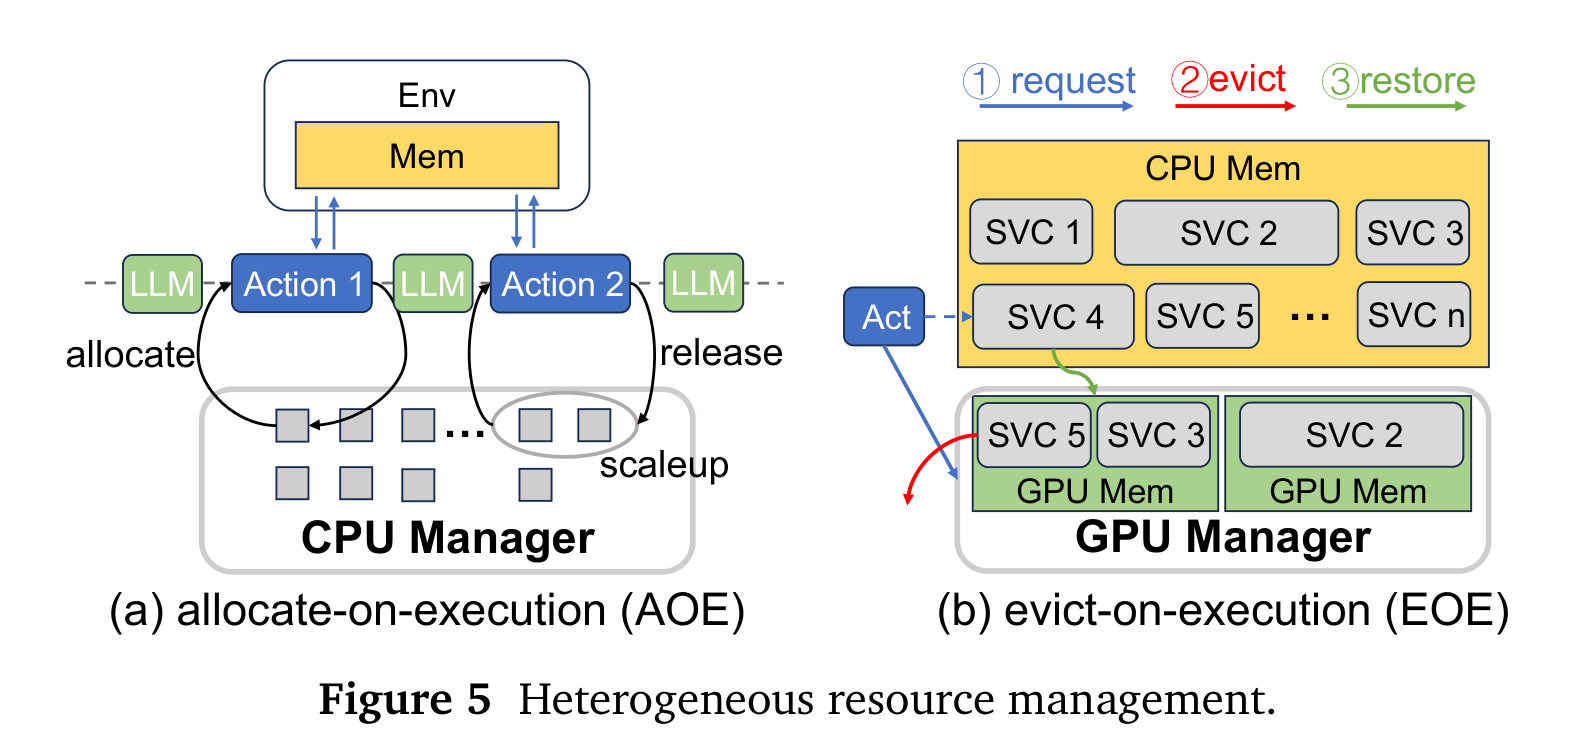
\includegraphics[width=0.85\textwidth]{figures/fig5.png}
\caption{异构资源管理机制示意。左图（a）为 AOE：CPU Manager 在每次 action 执行前动态分配 cgroup，action 完成后释放 CPU。右图（b）为 EOE：GPU Manager 维护多个 service 的 CPU 内存备份，按需将 service 恢复到 GPU 显存执行 action，完成后保持缓存直至被 LRU 淘汰。}
\label{fig:resource-mgmt}
\end{figure}

GPU reward service 的初始化开销（kernel 编译、通信组建立、模型参数加载至 GPU 内存）远高于 CPU 环境，无法简单地在每次 action 后完全释放和重建。EOE 的核心思路是将 GPU 显存作为多 service 的共享缓存，用 CPU 内存作为持久化存储。

\paragraph{Breakdown 机制（EOE）}
初始化时，GPU Manager 依次为所有 required service 分配 GPU，并将其状态备份到 CPU 内存。当 action 请求某 service 时：若该 service 已在 GPU 显存中，直接执行；否则从 CPU 内存恢复（restore），并根据需要驱逐（evict）其他 cached service 腾出显存。由于大多数 service 在调用间 GPU 内存状态不变，eviction 仅需释放 GPU 显存而无需写回 CPU 内存（CPU 内存中已有不变的副本），从而降低 context-switch 开销。

\paragraph{弹性 DoP}
将不同 DoP 配置的同一 service 视为不同的 service 实例，action 可被路由到任意 DoP 的实例，由调度算法决策。EOE 保证所有 cached service 有足够显存服务请求，每块 GPU 在任意时刻只执行一个 action。

\paragraph{Pool 机制：多级 chunk 结构}
GPU 集群的稀疏设备拓扑（节点内 GPU 少、并行度需求高）要求精细的碎片化管理。系统使用多级 chunk 结构管理 GPU 资源：合法分配集合（chunk）定义为满足~$\mathit{end} - \mathit{start} = 2^a$（$a \in \{0,1,2,3\}$）且~$\mathit{start}$ 能被~$2^a$ 整除的连续 GPU 区间。分配~$m$ 个 GPU 时（$2^{a-1} < m \leq 2^a$），按层级遍历可用 chunk，选取最小的满足条件的 chunk，若 chunk 过大则拆分。LRU 淘汰策略优先保留最近被请求的 service，当多个同级 chunk 可用时优先选择已缓存所请求 service 的 chunk 以减少 restore 开销。

\subsection{数据流与工作流}

以 AI coding rollout 为例的完整 action 处理流程：

\begin{enumerate}
  \item LLM 生成 shell command 后，RL 框架向 ARL-Tangram 提交 action（携带 trajectory ID、资源代价向量、弹性参数）；
  \item Formulation 模块记录 action 并将其入队；
  \item 调度器被触发（新 action 到达或现有 action 完成），从队列头部选取候选，运行贪心淘汰算法决定各 action 的 DoP；
  \item CPU Manager 通过 Docker API 更新对应容器的 cgroup（cpuset 指定所分配的核），fork 子进程执行 shell command；
  \item 执行完成，进程退出，CPU 资源回收；结果返回 RL 框架，LLM 继续下一轮生成。
\end{enumerate}

\subsection{技术栈与部署}

\begin{itemize}
  \item \textbf{RL 框架}：VeRL（Sheng et al., 2025），扩展了外部资源调用、sequence-level 和异步 rollout 能力；
  \item \textbf{CPU 集群}：15 个节点，每节点 256 个 AMD CPU 核、2.4~TB 内存；
  \item \textbf{GPU 集群}：5 个节点，每节点 8 块高端 NVIDIA GPU、3~TB CPU 内存；
  \item \textbf{RL 训练集群}：最多 48 个 GPU 节点，每节点 8 块 NVIDIA Hopper 架构 GPU，NVLink + RDMA 互联；
  \item \textbf{外部 API}：Google Search 至 PDF 解析服务等，均有 quota 约束；
  \item \textbf{系统独立性}：ARL-Tangram 作为独立系统部署，不与任何特定 RL 框架、外部资源类型或调用类型绑定。
\end{itemize}

% ============================================================
\section{实验设计与评估分析}
% ============================================================

\begin{keyinsight}[TL;DR]
在三种真实 agentic RL workload（AI Coding、MOPD、DeepSearch）上，ARL-Tangram 在 ACT、step duration 和资源节省三个维度上全面优于各专用基线，扩展性实验和消融实验进一步验证了弹性调度算法的有效性。
\end{keyinsight}

\subsection{实验配置}

\begin{table}[htbp]
\centering
\caption{实验配置概览}
\label{tab:expsetup}
\begin{tabular}{p{3.0cm}p{10.0cm}}
\toprule
\textbf{配置项} & \textbf{详情} \\
\midrule
数据集/Workload & AI Coding（in-house SWEBench-based，batch size 1280）；DeepSearch（BrowseComp，batch size 2048）；MOPD（batch size 2048）；MOPD+DeepSearch（并发，共 10 个 reward service） \\
基线系统 & AI Coding：Kubernetes（每 pod 0.5 CPU，上限 4 CPU）；MOPD：SGLang（9 教师模型，每模型 4 GPU with TP）；DeepSearch：各轨迹独立 API 调用（最多重试 3 次，600s timeout），5 个 reward 副本（TP=8）；GPU 扩展实验额外引入 ServerlessLLM \\
评估指标 & 平均 ACT（across time windows）；step duration（10 步均值）；各阶段时长分解（LLM/Tool/Reward，归一化到 ARL-Tangram 总时长） \\
计算资源 & RL 训练：最多 48 个 Hopper GPU 节点；CPU 外部资源：15 节点（256 AMD 核/节点）；GPU 外部资源：5 节点（8 GPU/节点） \\
关键超参数 & $\mathit{depth} = 2$；弹性 profile 提前离线采集（仅对 CPU reward 计算和 GPU reward model inference）；RL 训练模型：Qwen3-32B 和 MiMo-V2-Flash \\
\bottomrule
\end{tabular}
\end{table}

\subsection{核心实验结果}

\subsubsection{端到端性能（End-to-End Performance）}

\begin{figure}[htbp]
\centering
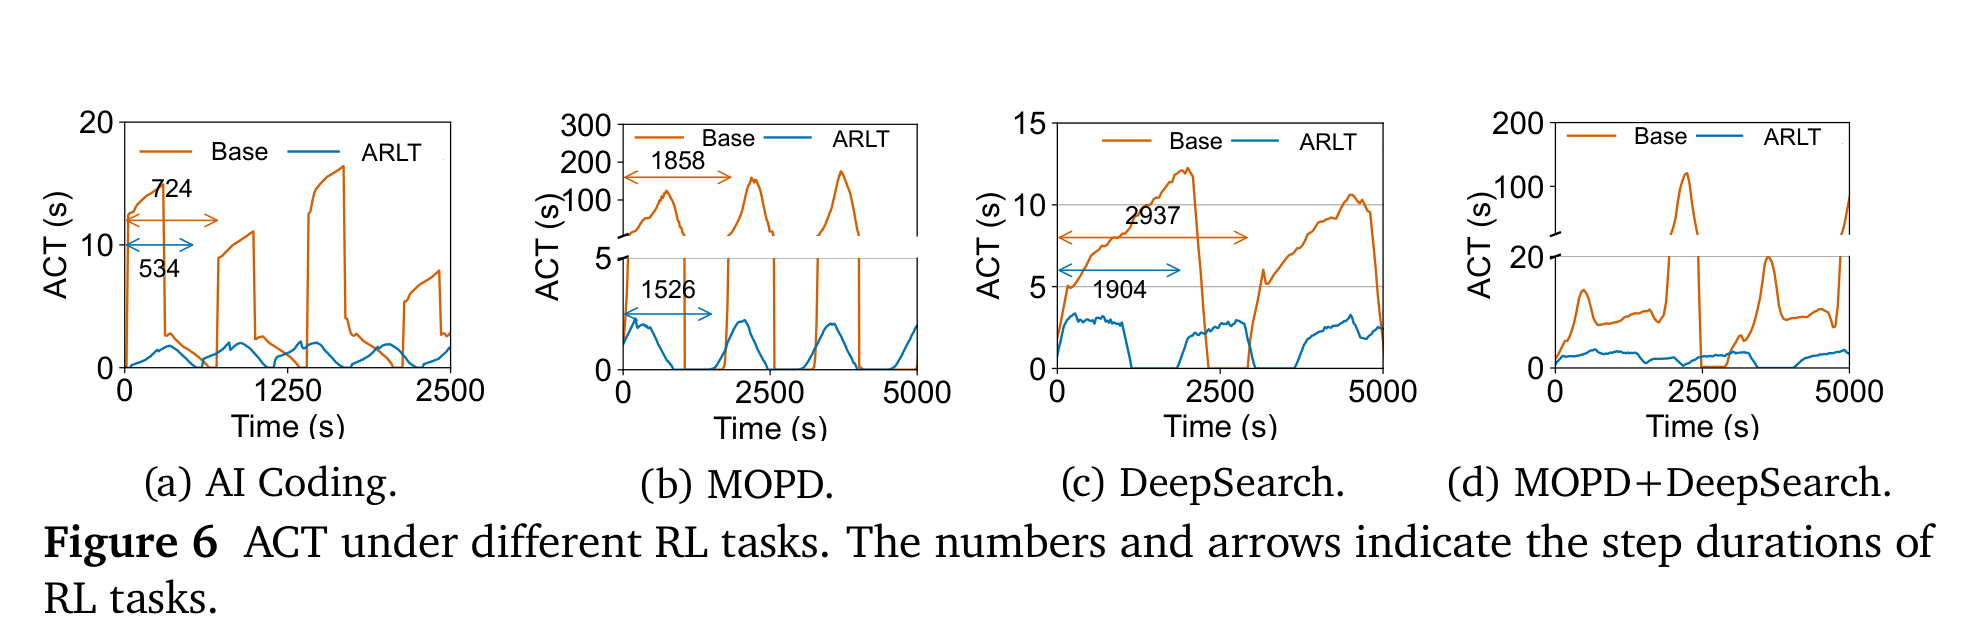
\includegraphics[width=\textwidth]{figures/fig6.png}
\caption{四种 RL task 下 ACT 随训练时间的变化（连续小时间窗口的均值）。ARL-Tangram（ARLT）在所有 workload 上始终低于基线。图中数字和箭头标注了各 RL task 的 step duration。}
\label{fig:act-curves}
\end{figure}

\begin{figure}[htbp]
\centering
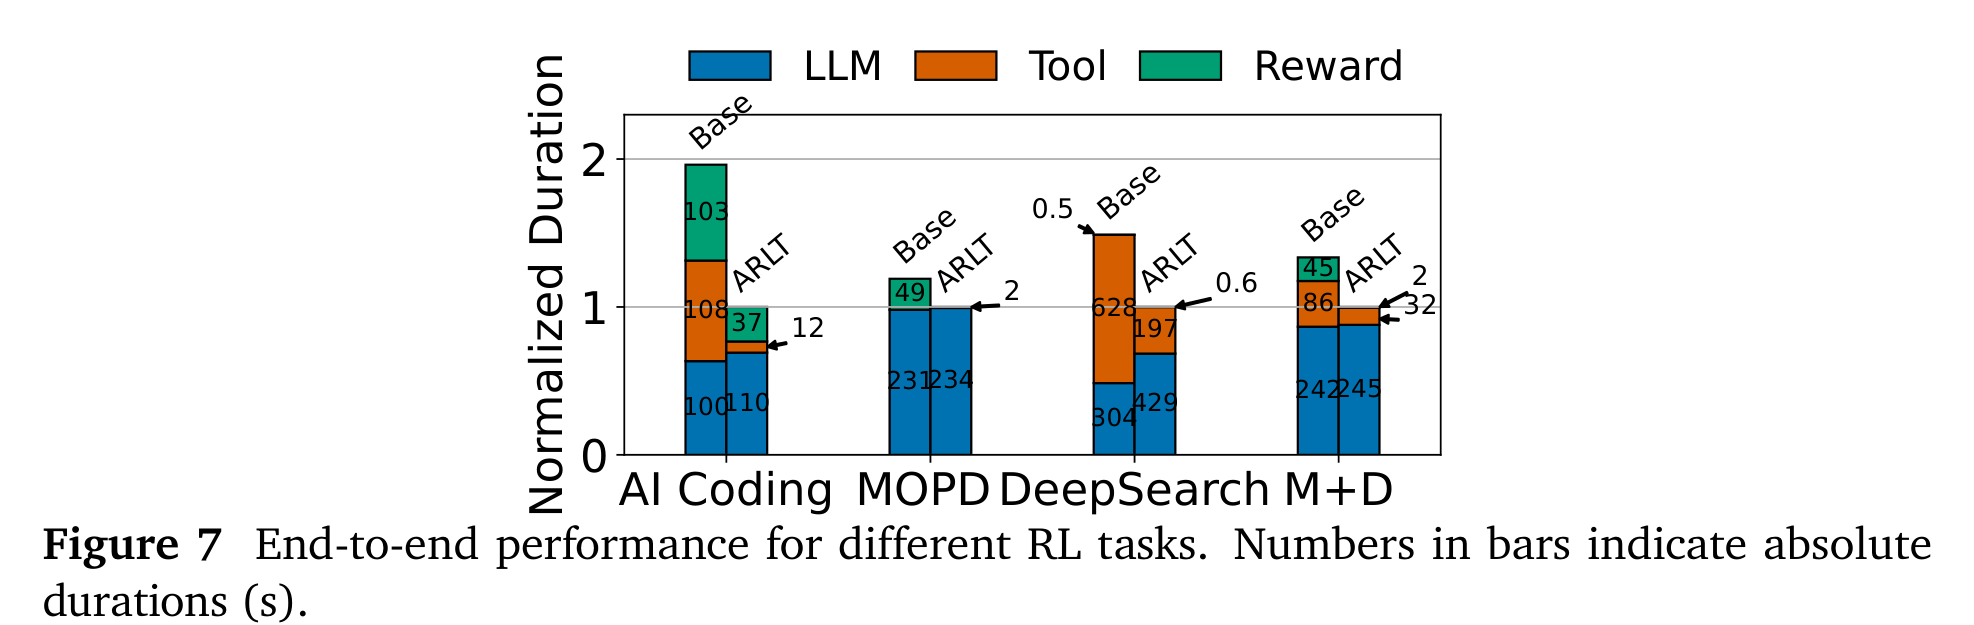
\includegraphics[width=0.9\textwidth]{figures/fig7.png}
\caption{不同 RL task 的端到端轨迹时长分解（LLM / Tool / Reward 三阶段，归一化到 ARL-Tangram 总时长）。柱中数字为绝对时长（秒）。}
\label{fig:e2e-breakdown}
\end{figure}

如图~\ref{fig:act-curves} 和图~\ref{fig:e2e-breakdown} 所示，核心结果如下：

\begin{itemize}
  \item \textbf{AI Coding}：环境交互时长降低~$9.0\times$（轨迹级 over-provisioning 消除，排队延迟减少），reward 计算时长降低~$2.8\times$（弹性 DoP 分配），外部调用总时长降低~$4.3\times$，step duration 提升~$1.4\times$；
  \item \textbf{MOPD}：通过跨 RL task 的教师模型共享和 GPU 资源池化，reward 时长显著降低；由于 MOPD 的 step duration 受 long-tail trajectory 主导，step duration 改善相对较小；
  \item \textbf{DeepSearch}：API 调用本身不可弹性扩展，ACT 改善主要来自流量控制（避免频繁 API failure 和重试），step duration 提升~$1.5\times$；
  \item \textbf{MOPD+DeepSearch（并发）}：在两种 workload 共享 GPU 集群时，ARL-Tangram 的 GPU 资源池化优势最为突出，相比各自独占资源的基线取得显著优势。
\end{itemize}

\begin{keyinsight}[DeepSearch 的特殊性]
DeepSearch 中 reward service（ARL-Tangram）的 reward 时长略高于基线（单模型场景，存在 restore overhead），但其 step duration 仍提升~$1.5\times$，原因是基线频繁的 API failure 降低了有效轨迹比例（pass rate），间接拉长了 step duration。这说明 ACT 改善并非 ARL-Tangram 价值的唯一来源，可靠性提升也是重要维度。
\end{keyinsight}

\subsubsection{系统扩展性（Scalability）}

\begin{figure}[htbp]
\centering
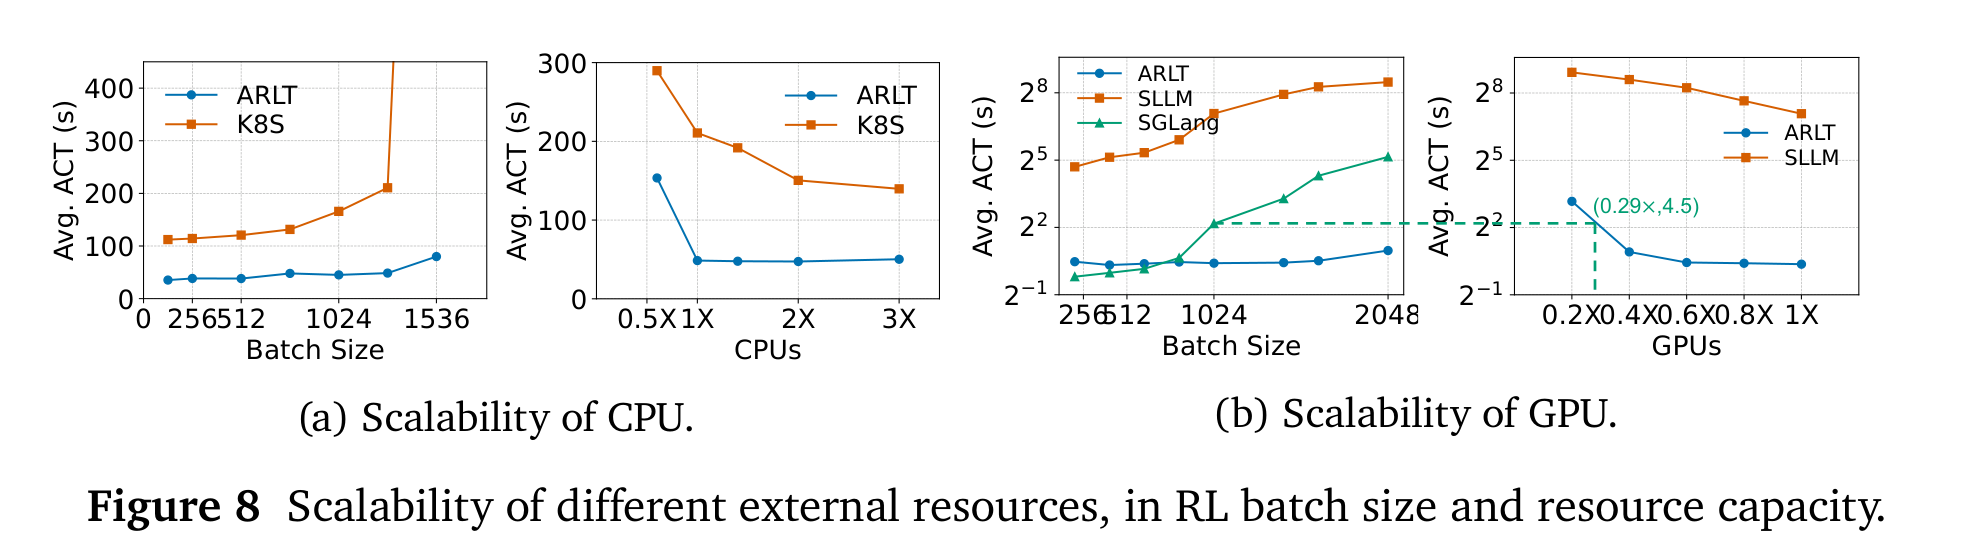
\includegraphics[width=\textwidth]{figures/fig8.png}
\caption{外部资源扩展性实验。上行为 CPU 扩展性（不同 batch size 和 CPU 核数配置），下行为 GPU 扩展性（不同 batch size 和 GPU 数量），对比 Kubernetes、SGLang 和 ServerlessLLM 基线。}
\label{fig:scalability}
\end{figure}

\paragraph{CPU 扩展性}
在 1280 个 CPU 核的固定配置下，随 RL batch size 增大，ARL-Tangram 将平均 ACT 提升~$3.1\times$ 至~$27.7\times$（相比 Kubernetes）。当 batch size 达到 1536 时，Kubernetes 控制面因资源不足触发频繁排队超时，而 ARL-Tangram 仅相比 batch size 128 时 ACT 增加不到~$2\times$，保持可用。在固定 batch size 为 1280、仅改变 CPU 核数的实验中，基线比 ARL-Tangram 慢~$1.89\times$ 至~$4.33\times$。

\paragraph{GPU 扩展性}
在 batch size 2048 下，ARL-Tangram 的平均 ACT 比 SGLang 低~$18.1\times$；ServerlessLLM 在该并发级别因超时失败率过高无法正常工作。在 batch size 1024 下，ARL-Tangram 优于 SGLang~$3.4\times$、优于 ServerlessLLM~$101.8\times$（注：低并发下 SGLang 因无 restore overhead 而略优于 ARL-Tangram）。在固定 batch size 1024、仅改变可用 GPU 数的实验中，ARL-Tangram 可用 29\% 的 GPU 数量服务 10 个 reward service 并达到相同 ACT，即节省 71\% 的外部 GPU 资源。

\subsection{消融实验分析}

\begin{figure}[htbp]
\centering
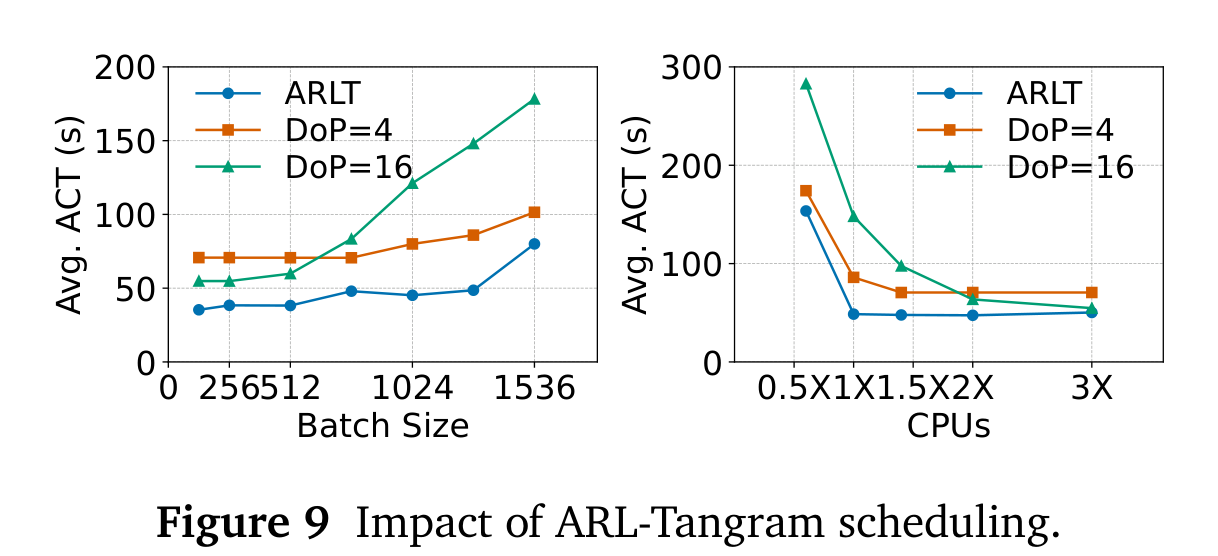
\includegraphics[width=0.85\textwidth]{figures/fig9.png}
\caption{弹性调度算法消融实验：与固定 DoP 基线（DoP=4 和 DoP=16）的 ACT 对比，在不同 batch size 和资源量条件下测试 AI Coding workload。}
\label{fig:ablation}
\end{figure}

以 AI Coding workload 为基础构建基于真实 RL trace 的 benchmark，对比弹性调度（DoP 范围 1-32）与固定 DoP 基线（DoP=4 和 DoP=16）：

\begin{itemize}
  \item 在 batch size 256 时，弹性调度相比 DoP=4 降低 ACT~$2.0\times$；
  \item 在 batch size 1280 时，弹性调度相比 DoP=16 降低 ACT~$3.0\times$；
  \item 在 1× CPU 资源受限场景下，弹性调度相比 DoP=4 实现~$1.8\times$ 改善。
\end{itemize}

这说明固定 DoP 策略对负载和资源变化的适应能力不足：DoP=4 在高并发时资源碎片化；DoP=16 在低并发时过度占用资源导致排队等待。弹性调度算法通过动态调整策略持续保持接近最优状态。

\subsection{系统开销分析}

\begin{table}[htbp]
\centering
\caption{ACT 分解分析（Table 1 原文数据，时长单位为秒）}
\label{tab:overhead}
\begin{tabular}{lcccc}
\toprule
\textbf{Workload (batch size)} & \textbf{执行时长} & \textbf{排队时长} & \textbf{系统开销} \\
\midrule
AI Coding (1280) & 0.975 & 0.015 & 0.024 \\
AI Coding (1536) & 1.206 & 0.428 & 0.036 \\
MOPD (2048)      & 0.621 & 0.081 & 0.201 \\
MOPD (3072)      & 0.705 & 15.05 & 0.240 \\
\bottomrule
\end{tabular}
\end{table}

\begin{keyinsight}[GPU 系统开销的可接受性]
MOPD 中系统开销（主要为 restore 时延）约占执行时长的 25\%，不可忽略。但关键在于：随并发度从 batch size 2048 增大到 3072，系统开销仅从 0.201s 增至 0.240s（增幅约 19\%），远低于排队时长的爆炸式增长（从 0.081s 到 15.05s，增幅近 200 倍）。这说明 ARL-Tangram 的开销具备良好的可扩展性，不随负载急剧恶化。
\end{keyinsight}

\subsection{实验方法学评估}

\begin{itemize}
  \item \textbf{统计显著性}：论文未报告方差或置信区间，仅给出均值数据，无法评估结果稳定性；
  \item \textbf{基线公平性}：各 workload 分别设计针对性基线（Kubernetes for CPU、SGLang for GPU），未使用统一基线，有助于对标最强现有方案，但跨 workload 比较需谨慎；
  \item \textbf{数据集代表性}：AI Coding 使用 in-house 数据集（声称"更全面"），但无法被外部独立验证，可复现性受限；DeepSearch 使用 BrowseComp（公开 benchmark），代表性较好；
  \item \textbf{缺失实验}：（1）未评估 ARL-Tangram 调度开销（scheduling latency 本身）随 action 到达率的变化；（2）未分析 depth 参数对调度质量的影响；（3）未评估 EOE restore 开销在不同模型大小下的变化规律。
\end{itemize}

% ============================================================
\section{批判性分析}
% ============================================================

\begin{keyinsight}[TL;DR]
ARL-Tangram 在工程实现和生产部署上表现突出，但作为系统论文，其理论贡献相对有限，部分设计决策的普适性有待进一步验证。
\end{keyinsight}

\subsection{技术优势}

\begin{strengthbox}
\begin{itemize}
  \item \gmark{问题定义精准}：对 agentic RL 中外部资源 over-provisioning 的两层分析（轨迹级 vs. 任务级）清晰有力，利用真实 profiling 数据（47\% 利用率、SM activity <3\%）量化问题严重性，说服力强。

  \item \gmark{系统独立性设计}：ARL-Tangram 不与特定 RL 框架、资源类型或调用类型绑定，作为独立中间层部署，具备良好的通用性和长期可维护性。这与专为特定场景（如仅处理 reward）设计的工作形成鲜明对比。

  \item \gmark{异构资源统一抽象}：通过向量化资源代价模型和标准化的 Resource Manager 接口，实现了 CPU、GPU、API quota 在统一调度框架下的协同管理，而无需为每类资源单独实现调度逻辑。

  \item \gmark{生产验证}：系统已部署于小米 MiMo 系列模型的真实 RL 训练，而非仅停留于实验室 benchmark，这一落地事实本身就是重要的技术可行性证明。

  \item \gmark{弹性 DoP 的 NUMA-aware CPU 分配}：CPU Manager 在弹性分配时优先选取同一 NUMA 节点内的 CPU 核，体现了对底层硬件拓扑的深度理解，这类工程细节在系统论文中往往容易被忽视。
\end{itemize}
\end{strengthbox}

\subsection{技术不足与局限性}

\begin{weaknessbox}
\begin{itemize}
  \item \rmark{EOE restore 开销未充分量化}：GPU Manager 的 restore 开销（约 25\% 执行时间）被轻描淡写为"acceptable"，但论文未提供不同模型大小、GPU 带宽条件下的 restore 时延数据，难以评估在更大模型（如 70B+）场景下是否仍可接受。

  \item \rmark{弹性建模依赖离线 profile}：弹性参数（$T_{\mathit{ori}}$、$E(m)$）需要提前 profile，这假设 action 的执行时长分布在训练过程中相对稳定。对于输出长度高度可变的 agentic RL（LLM 输出决定工具调用内容，进而影响执行时长），这一假设的有效性存疑，论文未讨论 profile 漂移的影响。

  \item \rmark{单一 DP 近似可能次优}：getApproximatedObjective 中对剩余 action 的 ACT 估计（以最低资源顺序插入 completion heap）是粗糙近似，在 action 间执行时长差异悬殊时可能导致显著的次优调度，但论文未提供最优解的对比实验来量化近似误差。

  \item \rmark{多 RL task 并发实验不足}：MOPD+DeepSearch 是唯一的多任务并发实验，且仅展示了 GPU 共享场景。CPU 资源在多 RL task 间的并发共享优势未被直接实验验证。

  \item \rmark{代码未开源，可复现性受限}：系统依赖私有生产集群和 in-house 数据集，外部研究者无法独立复现。
\end{itemize}
\end{weaknessbox}

\subsection{核心假设审视}

\begin{itemize}
  \item \textbf{假设1：action 的弹性由单一关键资源类型主导}——在 GPU action（并行度决定延迟）和 CPU action（测试并行度决定延迟）场景下合理，但对于同时跨 CPU-GPU 的混合 action（如边缘计算场景）可能失效。

  \item \textbf{假设2：FCFS 执行顺序已足够避免 starvation}——FCFS 本身不完全防止 starvation（后来的短 action 可能因前面长 action 排队而饥饿），论文的论证基于「所有 action 在轨迹关键路径上所以都重要」，但不同 action 的紧迫程度可能确实存在差异（如 reward 计算 vs. 中间工具调用）。

  \item \textbf{假设3：EOE eviction 不需要写回 CPU 内存}——依赖于 service 的 GPU 内存状态在调用间不变，这对 stateless reward model 成立，但对 stateful service（如维持会话状态的 agent environment）不成立。

  \item \textbf{假设4：GPU chunk 大小限制为 $\{1,2,4,8\}$}——这限制了单个 action 的最大 GPU 数为 8（即一个节点），对于需要多节点 tensor parallelism 的超大 reward model 不适用。
\end{itemize}

\subsection{潜在失效模式}

\begin{itemize}
  \item \textbf{Profile 不准确场景}：若 action 执行时长分布因 LLM 输出模式改变而发生大幅漂移（例如，训练后期模型输出更长、更复杂的代码），基于历史 profile 的弹性估计将失效，调度决策趋向次优。

  \item \textbf{极端 bursty 负载}：当 action 提交速率远超系统处理能力时（如 MOPD batch size 3072 时排队时长达 15s），ARL-Tangram 虽能维持稳定，但绝对 ACT 仍然很大，此时弹性调度的改善空间有限（受限于物理资源）。

  \item \textbf{异构资源缺乏协同调度}：当 CPU 和 GPU 资源同时紧张且同一 action 需要两类资源时，分别管理可能导致 CPU 或 GPU 先到位但另一类资源未就绪的 partial allocation 问题，论文未明确说明如何处理。
\end{itemize}

\subsection{可复现性评估}

论文提供了充分的系统设计细节（算法伪代码、关键接口定义、chunk 结构数学描述），使得有意复现的研究团队可以基于相同思路实现系统。然而，代码未开源，testbed 为私有生产集群，in-house AI Coding 数据集不公开，使得精确数字复现不可行。BrowseComp（DeepSearch 数据集）为公开 benchmark，是唯一可被独立验证的评估场景。

% ============================================================
\section{数学与算法深入分析}
% ============================================================

\begin{keyinsight}[TL;DR]
论文的数学核心在于将 action 资源分配问题归约为多维 bin packing 的变体，并通过拓扑无关的 DP 框架和贪心淘汰算法在多项式时间内求近似最优解。
\end{keyinsight}

\subsection{核心公式分析}

\subsubsection{弹性函数的设计}

公式~(\ref{eq:elasticity})~$a.\mathit{getDur}(m) = T_{\mathit{ori}} / (E(m) \cdot m)$ 的直觉：
\begin{itemize}
  \item 若~$E(m) = 1$（完美线性加速），则~$\mathit{getDur}(m) = T_{\mathit{ori}} / m$，与理想并行加速比一致；
  \item 若~$E(m) < 1$（存在并行开销），则实际加速低于线性，体现 Amdahl 定律；
  \item 约束~$0 < E(m) \leq 1$ 排除了超线性加速的不合理情况；
  \item 设计上选择 $E(m)$ 为函数而非单一参数，允许非线性弹性曲线（如 GPU scaling efficiency 在小并行度时接近 1，大并行度时因 all-reduce 开销下降）。
\end{itemize}

\subsubsection{ACT 近似目标的分解}

getApproximatedObjective 将 ACT 分解为两部分：

\begin{mathbox}[ACT 近似目标分解]
\begin{equation}
  \mathit{approxACT} = \underbrace{\mathit{exactObj}}_{\text{candidate 精确 ACT（DPArrange 求解）}} + \underbrace{\mathit{approxObj}}_{\text{剩余 action 近似 ACT（min 资源+顺序插入估计）}}
\end{equation}
\end{mathbox}

精确部分通过 DPArrange 求得 optimal allocation，近似部分通过 depth 参数控制第一个剩余 action 的多分配策略探索，在精度和计算开销间取得平衡。

\subsection{算法描述}

核心弹性调度算法（Algorithm 1）的关键设计：

\begin{itemize}
  \item \textbf{候选选择（Line 1-2）}：$n = \max\{i \mid R.\mathit{accommodate}(W[:i])\}$，即在资源约束（含拓扑约束）下能以最低资源同时容纳的最多 action 数；
  \item \textbf{资源类型分组（Line 3-4）}：$C_j = C.\mathit{split}(R_j)$，将候选按关键弹性资源分组，不同组独立处理（单资源弹性假设保证不同维度间无耦合）；
  \item \textbf{贪心淘汰（Line 8-11）}：从~$t=1$ 开始逐步淘汰末尾 action，每次比较淘汰后 objective 是否改善，一旦不改善立即终止，避免盲目驱逐。
\end{itemize}

\subsection{复杂度分析}

\begin{itemize}
  \item \textbf{调度算法整体}：$O(kn^2m^2)$，其中~$k$ 为资源类型数，$n$ 为候选数，$m$ 为单类资源剩余 unit 数。在 GPU 场景中~$k=1$，$n$ 和~$m$ 受限于集群规模（实践中较小），保证了毫秒级的调度开销；
  \item \textbf{DPArrange（Algorithm 3）}：$O(m \cdot n \cdot |S|)$，其中~$|S|$ 为支持的分配量集合大小。对 GPU chunk 结构（$|S| \leq 4$），复杂度为~$O(mn)$；
  \item \textbf{GPU chunk DP 状态空间}：$(N_1+1)(N_2+1)(N_4+1)(N_8+1)$，mixed-radix 编码保证状态的唯一映射和有限 DP 空间。
\end{itemize}

\subsection{理论分析}

论文引用 Bruno et al. (1974) 指出，将有限资源在弹性 job 间分配以最小化 total JCT 是 NP-hard 问题，因此选择启发式算法有充分的理论依据。然而，论文未提供贪心淘汰算法的近似比分析，无法量化其与最优解的差距。对于实践中最关键的问题——「贪心淘汰在多大程度上接近最优？」——仅靠与固定 DoP 基线的比较无法完整回答。

% ============================================================
\section{结论与未来展望}
% ============================================================

\begin{keyinsight}[TL;DR]
ARL-Tangram 将云计算资源弹性管理的成熟思想引入 agentic RL 的关键基础设施层，已通过生产部署验证其有效性，未来在更广泛的 agentic 场景和更复杂的异构资源拓扑下仍有大量工作可做。
\end{keyinsight}

\subsection{核心结论}

ARL-Tangram 的核心贡献在于正确识别了 agentic RL 外部资源管理的粒度错配问题——现有框架用轨迹/任务级管理面对 action 级的资源需求模式，必然导致 over-provisioning。通过将管理粒度细化到 action 级，系统同时实现了资源利用率的提升（pool）和延迟的降低（弹性 DoP）。AOE 和 EOE 两种机制分别针对 CPU 和 GPU 的异构特性，展现了良好的工程实用主义：CPU 环境状态廉价（仅需保留内存），故用 cgroup 动态分配即可；GPU 服务状态昂贵（完整加载模型），故用 CPU 内存作为低成本备份存储。

\subsection{实践意义与设计启示}

\begin{itemize}
  \item \textbf{设计启示1：外部资源管理不应是 RL 框架的"二等公民"}：agentic RL 的外部调用在关键路径上，其延迟直接决定 rollout 效率和 GPU 训练集群利用率，应与主训练集群的调度设计同等重视；
  \item \textbf{设计启示2：Breakdown 优先于 Pool}：减少每个调用占用资源的时间（breakdown）是 Pool（共享资源）的前提；在没有 breakdown 的情况下，pool 只能作用于任务间隙，效果有限；
  \item \textbf{设计启示3：弹性调度需要 profile 支撑}：离线 profile 是弹性调度算法发挥效果的关键，工程团队在部署时应将 profile 采集作为标准流程；
  \item \textbf{工程注意事项}：EOE 的 restore overhead 在单服务低并发场景会反超原有部署（DeepSearch 中 reward time 略高于基线），需要评估并发度阈值才能决定是否启用 EOE。
\end{itemize}

\subsection{局限性与未来方向}

\subsubsection{作者提出的未来方向}
原文未明确讨论未来工作方向，结论部分仅总结了已有贡献。

\subsubsection{建议的研究方向}

\begin{enumerate}
  \item \textbf{Online 弹性 profile 与自适应调度}：现有系统依赖离线 profile，对训练过程中 action 特征漂移（LLM 能力提升导致更长、更复杂的工具调用）缺乏适应性。引入在线 profile 更新机制，结合 Bayesian 优化或 RL 自身来自适应调整弹性参数，是自然的扩展方向。

  \item \textbf{跨集群异构资源的联合调度}：当前 ARL-Tangram 的调度器在单一系统内运行，而超大规模 agentic RL（如多 datacenter 分布式训练）需要跨地理位置、跨云厂商的外部资源协同调度，涉及网络延迟建模和资源异构性的扩展。

  \item \textbf{与 RL 算法的协同优化}：ARL-Tangram 与 RL 框架解耦，虽然提高了通用性，但也错失了协同优化的机会。例如，若调度器了解当前 rollout 的优先级（高奖励的轨迹更值得加速），可以实现 reward-aware action scheduling，将外部资源优先给予最有价值的轨迹。
\end{enumerate}

% ============================================================
\section{延伸阅读建议}
% ============================================================

\begin{keyinsight}[TL;DR]
理解 ARL-Tangram 需要以 agentic RL 训练框架为基础，以资源调度理论为工具；进一步深入需要了解 LLM serving 系统和 GPU 显存管理领域的前沿工作。
\end{keyinsight}

\subsection{前置阅读（理解本文的基础）}

\begin{itemize}
  \item \textbf{HybridFlow/VeRL}（Sheng et al., 2025, EuroSys）：本文主要集成的 RL 框架，理解其 rollout/train 架构有助于定位 ARL-Tangram 的接入位置——[基础性/方法论基础]

  \item \textbf{ReAct}（Yao et al., 2022, ICLR）：agentic LLM 的基础 ReAct 模式（推理与行动交替），是理解 multi-turn tool invocation 为何成为关键路径的概念基础——[问题背景]

  \item \textbf{DeepSeek-R1}（Guo et al., 2025）：代表性的 RLVR 训练工作，理解 ground-truth reward 对 CPU reward 计算的外部资源需求——[问题背景]

  \item \textbf{GRAPHENE}（Grandl et al., 2016, USENIX OSDI）：数据并行集群中 packing+dependency-aware 调度，是文中引用的经典集群调度工作，提供 JCT 优化问题的基础方法论——[方法论基础]

  \item \textbf{HiveD}（Zhao et al., 2020, USENIX OSDI）：GPU 集群 sharing 框架，本文 GPU Manager 的 multi-level chunk 结构直接引用了 HiveD 的设计——[方法论基础]
\end{itemize}

\subsection{后续阅读（本文之后的进展）}

\begin{itemize}
  \item \textbf{Mars}（Zhu et al., 2026, USENIX NSDI）：专注 reward service 的高效化，与 ARL-Tangram 方法互补，可深入理解 reward 计算端到端优化——[竞争方案/扩展]

  \item \textbf{MegaFlow}（Zhang et al., 2026）：大规模分布式 agentic orchestration 系统，从 agent workflow 整体编排视角看外部资源管理问题——[扩展]

  \item \textbf{Aegaeon}（Xiang et al., 2025, ACM SOSP）：面向并发 LLM serving 的 GPU pooling 框架，GPU Manager EOE 机制可与该工作对比，理解 GPU 显存管理的不同设计取舍——[改进/竞争方案]

  \item \textbf{AReaL}（Fu et al., 2025）：异步 RL 框架，从 RL 算法层面减少 rollout 阻塞，与 ARL-Tangram 在系统层面的工作正交，两者结合可能实现更大提升——[扩展/互补]

  \item \textbf{MiMo-V2-Flash}（Xiao et al., 2026）：ARL-Tangram 实际服务的 RL 训练对象，可了解真实生产场景下 agentic RL 的规模与需求——[应用背景]
\end{itemize}

\end{document}
